% A short paper, of the shape this week's experiment was designed to fill.

% the files accuracy.pdf, table1.tex, table2.tex are the outputs from our W09 exercises. When you've made new versions of your own, drag them into the File panel on the left.

\documentclass[11pt,a4paper]{article}

\usepackage[margin=2.5cm]{geometry}
\usepackage{booktabs}   % \toprule, \midrule, \bottomrule: what pandas emits
\usepackage{graphicx}   % \includegraphics
\usepackage{natbib}

\title{Classifying \emph{Pygoscelis} penguins' sex from four body measurements:
       a comparison of nearest-neighbour classifiers}

% YOUR NAME GOES HERE. This is the one line of this file you have to change.
\author{A. Student \\ \small University of Galway}

\date{\today}

\begin{document}
\maketitle

\begin{abstract}
Since the dawn of time, humans have wondered whether it is possible to
tell whether a penguin is male or female based only on body size and 
length of bill. We consider this urgent question.
We find that normalising the measurements matters a great deal, that the
choice of distance metric does not matter at all, and that adding the
categorical columns such as island of origin makes matters slightly worse.
\end{abstract}

\section{Introduction}

Instead of an introduction, please just read the abstract twice.

\section{Data and method}

According to Horst et al., body size measurements
were collected for ``three species of {\em Pygoscelis} penguins that breed on islands throughout the Palmer Archipelago, Antarctica''~\citep{horst2022palmer}. The original data was published as~\citet{horst2020palmer}.
Three hundred and forty-four penguins were measured, of which 333 were also
sexed, i.e.~their sex was determined.

In our methodology, the remaining eleven are dropped, 
because a missing label cannot be
imputed. We hold out 20\% of the sexed birds as a test set, touch it once,
and do everything else --- choosing $k$, the metric, whether to normalise and
which columns to use --- on the remaining 266 by five-fold cross-validation
repeated five times, giving 25 train/test splits per configuration.

\section{Results}

Table~\ref{tab:baselines} gives the models we have to beat. A classifier that
always answers with the commoner label scores 0.504, which is the number
every other number in this paper should be read against.

\begin{table}[!htbp]
  \centering
  \begin{tabular}{lrrrr}
\toprule
setting & cats off, norm off & cats off, norm on & cats on, norm off & cats on, norm on \\
model &  &  &  &  \\
\midrule
Dummy (most frequent) & 0.504 & 0.504 & 0.504 & 0.504 \\
Decision tree & 0.847 & 0.849 & 0.851 & 0.852 \\
Random forest & 0.897 & 0.898 & 0.901 & 0.902 \\
\bottomrule
\end{tabular}

  \caption{Accuracy of three reference models, averaged over 25 train/test
    splits. The two tree models are unaffected by normalisation, as they
    must be: a tree compares one feature against a threshold, and rescaling
    a column cannot change which side of it a bird falls.}
  \label{tab:baselines}
\end{table}

Table~\ref{tab:factorial} gives the full factorial, and
Figure~\ref{fig:accuracy} the same numbers with their error bars.

\begin{table}[!htbp]
  \centering
  \small\begin{tabular}{llrrrr}
\toprule
 & setting & cats off, norm off & cats off, norm on & cats on, norm off & cats on, norm on \\
metric & k &  &  &  &  \\
\midrule
chebyshev & 1 & 0.722 & 0.875 & 0.722 & 0.880 \\
 & 3 & 0.709 & 0.898 & 0.709 & 0.881 \\
 & 5 & 0.721 & 0.905 & 0.721 & 0.895 \\
 & 9 & 0.742 & 0.905 & 0.742 & 0.899 \\
 & 15 & 0.738 & 0.901 & 0.738 & 0.895 \\
 & 25 & 0.744 & 0.893 & 0.744 & 0.827 \\
 & 45 & 0.756 & 0.856 & 0.756 & 0.702 \\
euclidean & 1 & 0.728 & 0.865 & 0.730 & 0.872 \\
 & 3 & 0.737 & 0.898 & 0.737 & 0.891 \\
 & 5 & 0.759 & 0.919 & 0.759 & 0.905 \\
 & 9 & 0.751 & 0.905 & 0.751 & 0.900 \\
 & 15 & 0.750 & 0.891 & 0.750 & 0.900 \\
 & 25 & 0.756 & 0.900 & 0.756 & 0.850 \\
 & 45 & 0.764 & 0.880 & 0.762 & 0.822 \\
manhattan & 1 & 0.751 & 0.875 & 0.757 & 0.878 \\
 & 3 & 0.746 & 0.894 & 0.752 & 0.890 \\
 & 5 & 0.761 & 0.899 & 0.759 & 0.897 \\
 & 9 & 0.752 & 0.910 & 0.754 & 0.893 \\
 & 15 & 0.755 & 0.895 & 0.756 & 0.894 \\
 & 25 & 0.759 & 0.890 & 0.758 & 0.850 \\
 & 45 & 0.763 & 0.878 & 0.764 & 0.818 \\
\bottomrule
\end{tabular}

  \caption{Accuracy of our nearest-neighbour classifier at every combination
    of the four factors, averaged over 25 train/test splits. Normalisation
    is worth roughly twelve points; the three metrics are indistinguishable;
    accuracy peaks around $k=5$ and falls away on either side.}
  \label{tab:factorial}
\end{table}

\begin{figure}[!htbp]
  \centering
  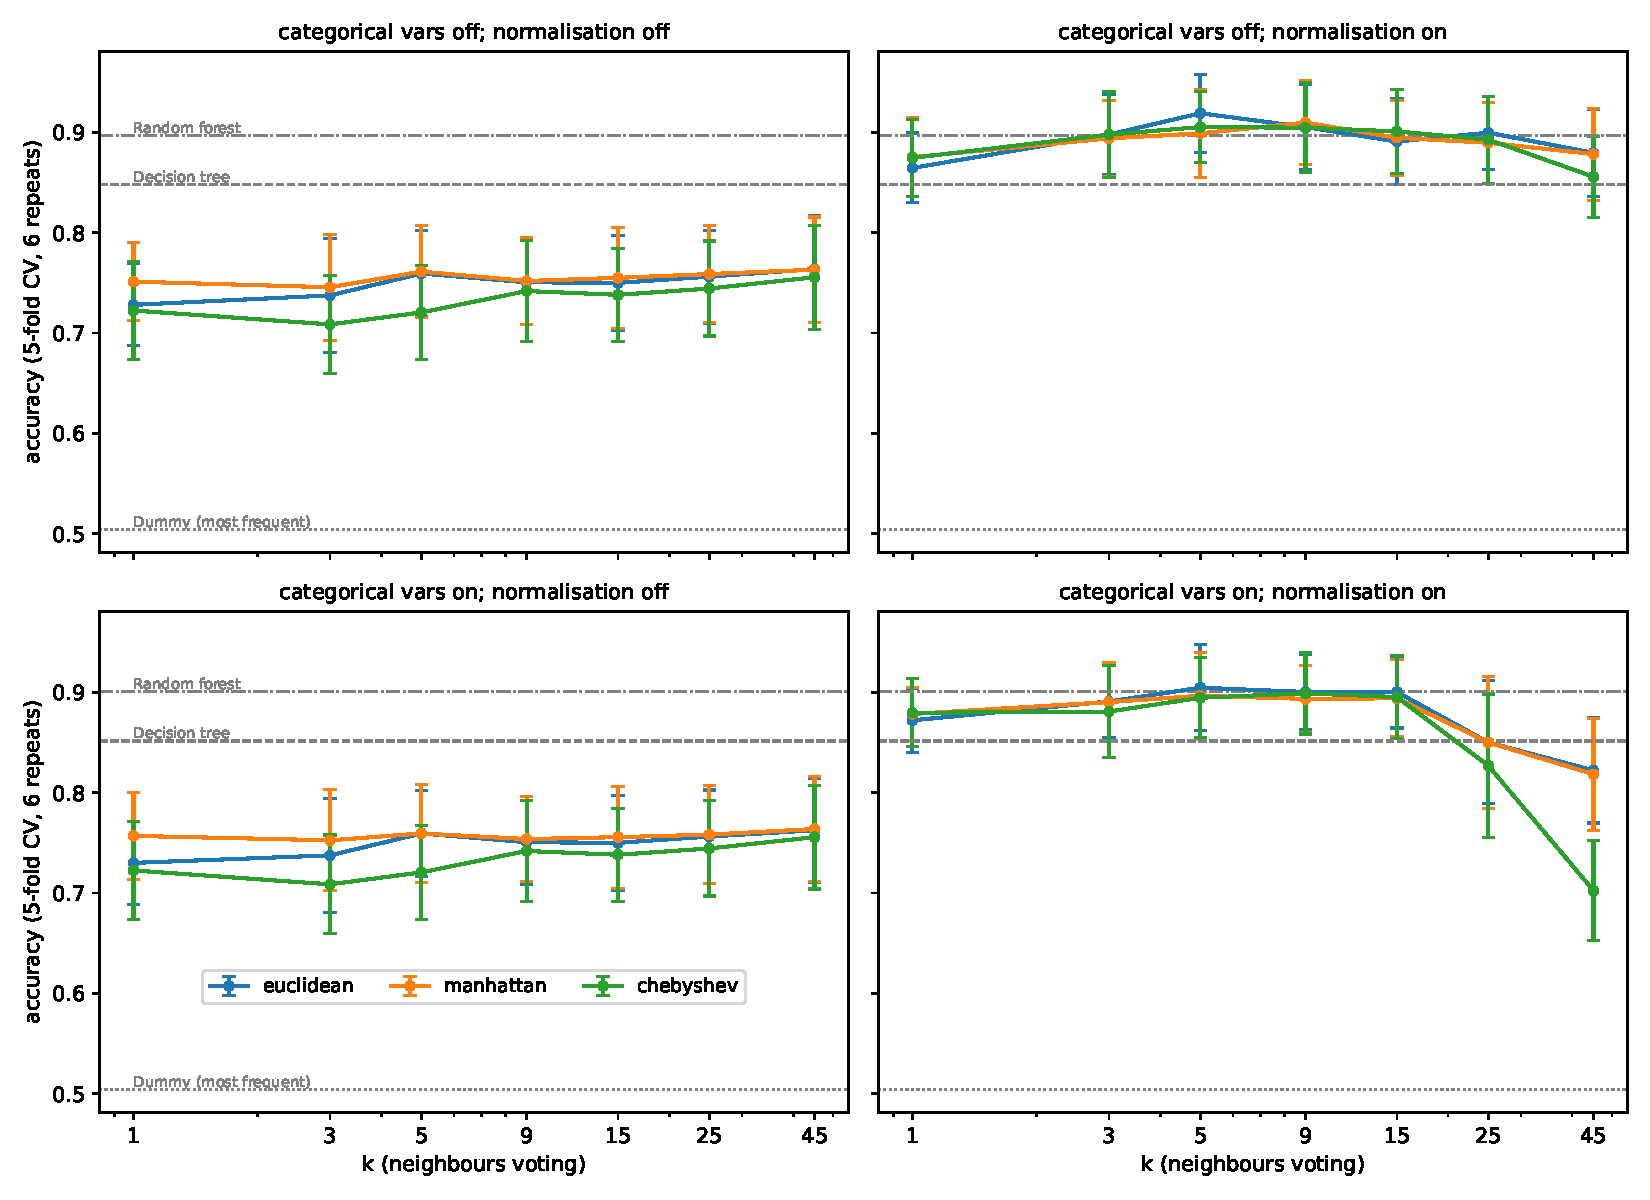
\includegraphics[width=0.78\textwidth]{accuracy.pdf}
  \caption{Accuracy against the number of voting neighbours $k$, for each
    combination of feature set and normalisation, with one line per distance
    metric. Error bars are one standard deviation across the 25 splits;
    horizontal lines mark the reference models of
    Table~\ref{tab:baselines}. Note that the categorical columns change
    nothing while the features are unnormalised --- a zero-or-one column
    contributes almost nothing to a distance dominated by body mass in grams
    --- and start doing harm as soon as they are given equal weight.}
  \label{fig:accuracy}
\end{figure}

\section{Conclusions}

It is now time to end this paper.

\section{Ethics statement}

No penguins were harmed during this computational experiment, but we
are not entirely sure about the original data-gathering.


\bibliographystyle{plainnat}
\bibliography{refs}

\end{document}
